%%
%% neuralfields.tex
%% 
%% Made by jjfigueredou
%% Login   <jjfigueredou@fctp-jjfu>
%% 
%% Started on  Sun Oct  5 12:26:22 2008 jjfigueredou
%% Last update Sun Oct  5 12:26:22 2008 jjfigueredou
%%

\documentclass{sig-alt-release2}

\usepackage{algorithm}
\usepackage{algorithmic}

\begin{document}

\conferenceinfo{GECCO'09,} {July 8--12, 2009, Montr\'eal Qu\'ebec,
  Canada.}

\CopyrightYear{2009}

\crdata{978-1-60558-325-9/09/07}
%
% --- Author Metadata here --- \conferenceinfo{WOODSTOCK}{'97 El Paso,
%   Texas USA}
% \CopyrightYear{2007} % Allows default copyright year (200X) to be over-ridden - IF NEED BE.
% \crdata{0-12345-67-8/90/01} % Allows default copyright data (0-89791-88-6/97/05) to be over-ridden - IF NEED BE.
% --- End of Author Metadata ---

\title{Evolved Neural Fields Applied to the Stability Problem of a
  Simple Biped Walking Model}

\numberofauthors{1}
\author{\alignauthor Juan J. Figueredo, Jonatan G�mez \\
  \affaddr{Universidad Nacional de Colombia}
  \\ \affaddr{ Ciudad Universitaria, Bogot�, Colombia} \\
  \email{jjfigueredou@unal.edu.co, jgomezpe@unal.edu.co} }

\maketitle

\begin{abstract}
  This paper proposes an evolved control architecture based on neural
  fields for a relatively complex and unstable dynamical system. The
  neural field model is capable of addressing goal-based planning
  problems and has properties, like embedding in an Euclidean space
  and linear stability, that potentially make it well-fitted for
  dynamic control tasks. The neural field control architecture is
  tested over the stability problem on a typical inverted-pendulum and
  the performance of an evolved neural field and a hand-tuned neural
  field is compared. The neural field controller performs well in the
  simulation and has a spatial representation which allows
  interpretation of field potentials. Also, the evolved neural field
  performs better than the non-evolved one, uses a different strategy
  to control the plant, and is able to recover faster from worst-case
  initial conditions.
\end{abstract}

\vspace{1mm}
\noindent {\bf Categories and Subject Descriptors:} I.2.8 {Artificial
  Intelligence}: {Problem Solving, Control Methods, and Search}

\vspace{1mm}
\noindent {\bf General Terms:} Algorithms, Design.

\vspace{1mm}
\noindent {\bf Keywords:} Neural fields, neurocontrol, evolutionary
robotics, artificial life.

\section{Introduction}
In biped robotics, the methods based on computational intelligence for
planning and control have shown to be able to achieve static stability
\cite{Kun97Adaptive}, dynamical stability
\cite{Nakanishi2004b,Komatsu05Dynamic}, achieve simple control
structures \cite{Huelse04Structure}, and tolerate perturbations
\cite{Juang02Intelligent}. Nonetheless, those properties have not been
extended to an integrated architecture of planning and control capable
of following goals.

Here a control scheme based on neural fields is proposed and a
comparison, on the stability problem of an inverted pendulum, is made
between a hand-tuned controller and a controller parameterized by an
evolutionary algorithm. As controllers, the neural fields, compared
with recurrent neural networks, have a deeper biological basis, apply
more restrictions and extend the discrete model to a continuous one,
following the method of planning and control by means of neural fields
\cite{Bergener99Complex}. The neural field model, as noted in the
article by Bergener et al., has the potential to address goal-based
planning problems, so we are here interested on its capability to
solve dynamic control problems.

\subsection{Neural Fields}
Neural fields arise as a tissue level model of neural populations in
brain. They have been proposed by Wilson and Cowan
\cite{Wilson72Excitatory} and detailed by Amari \cite{Amari77Dynamics}
in the particular case of lateral inhibition. In this model, a neural
population is considered a continuum in which dynamical evolution is
driven by mean activation potentials. The field potential is evaluated
in each place and affected by the neighborhood of that place,
according to a so-called mexican hat function (as noted by Coombes
\cite{Coombes05Waves} better called wizard hat function), in which
close neighbors act as exciters and distant ones act as
inhibitors. The elements on the field are embedded into a metric
space, usually a one-dimensional or two-dimensional Euclidean space.
\subsection{The Stability Problem Model}
\label{sec:model}

The model used consists of an approach to biped walking based on a
inverted pendulum (car-and-pole) system in which the pendulum
equilibrium is looked for. The dynamic model used, in mathematical
terms, is expressed in the two equations:

\begin{align}
  \label{eq:nf-simp}
  \ddot{x}&=\frac{F+ml\dot{\theta}^2\sin\theta-mg\cos\theta\sin\theta}{M+m\sin^2\theta}\\
  \ddot{\theta}&=\frac{(M+m)g\sin\theta-F\cos\theta-ml\dot{\theta}^2\sin\theta\cos\theta}{l(M+m\sin^2\theta)}+\frac{\tau}{ml^2}-\frac{\dot{\theta}}{2}
\end{align}
Where $x$ here is the linear position, $\theta$ is the angular
position, $M$ is the pendulum mass (located at the outer side), $m$ is
the cart mass, $l$ is the pendulum length and $g$ is the gravity
acceleration. It is included in the model a viscous friction for the
rotation.

\section{Neural Fields for Control and Planning}

The proposed control architecture based on the neural fields has three
basic elements: A sensor which reads the states from the plant and
also their derivatives (computed from the dynamical equation of the
plant). In particular, the sensor used for the neural field controller
is rather simple, taking the values of the angular-related states
(i.e. angular position and angular velocity) as feedback. An input
layer that consists of a simple neural field without natural dynamics
and produces a spatial codification of the sensed values. For the
problem at hand, we use a finite one-dimensional neural field, where a
sensed input with value zero maps to the center point of the field,
and other values are correspondingly coded in other (positive or
negative) positions. Angular position values are coded as local
potentials with value $u(x)=1$ and angular velocities as local
potentials with value $u(x)=k_\omega$, where $0 \le k_\omega < 1$. It
is worth noting that the sum between input states is performed
directly by the neural field dynamics. A processing layer which is a
more typical neural field which has inner dynamics given by the
equation \ref{eq:nf-disc}. Each position of the processing field takes
as input, both the field potentials of the processing field, and the
field potentials of the input field. Therefore, besides its natural
dynamics, the processing layer receives the inputs from the input
field filtered by the kernel operator. The kernel operator used here
is a Wizard Hat Function with the expression shown in equation
\ref{eq:wizard-hat}:

\begin{equation}
  \label{eq:wizard-hat}
  w(x_i,x_j)=ke^{-(x_i-x_j)^2/\delta^2}-H_0
\end{equation}

The additional term on the eq. \ref{eq:nf-disc} $S(x_i,t)$ is used
only as the uniform and static resting potential, that is
$S(x_i,t)=-r_p$.  The firing rate function $f(u_i)$ is simulated as a
simple Heaviside function. The kernel operator for the
evolutionary-tuned case is evaluated with the expression:

\begin{equation}
  w(x_i,x_j)=\mathtt{kernelArray}[|x_i-x_j|]
\end{equation}

Where \texttt{kernelArray} is the array of parameters modified by the
evolutionary algorithm. The kernel value is evaluated by accessing the
array at position $|x_i-x_j|$.

The additional term on the eq. \ref{eq:nf-disc} $S(x_i,t)$ is used
only as the uniform and static resting potential, that is
$S(x_i,t)=-r_p$.  The firing rate function $f(u_i)$ is simulated as a
simple Heaviside function.

The output is processed taking the position with highest activation on
the processing filtered by another wizard-hat function, and decoding
it to a value.

\section{Evolution of Neural Field Controllers}
We used a simple evolutionary algorithm, with random elimination of
individuals inversely proportional with their fitness. The evolution
parameters are the connection kernels between the input layer and the
processing layer, and the recurrent connections of the processing
layer with itself. The connection kernels are considered isotropic and
homogeneous along the field, so that they can be described as
symmetric one-dimensional arrays of values. Each connection kernel can
be represented as an array of $N$ values from $w(0)$ to $w(n)$ with
homogeneous spacing, using their symmetry. Therefore, for an equal
boundary radius for all the kernels, and a 2-layered architecture,
there are $2N$ real values in the genotype. The evolution operations
used in both steps are:
\begin{itemize}
\item Gaussian modification of real codified array values, which
  varies the connection kernel between input layer and processing
  layer.
\item Gaussian modification of real codified array values, which
  varies the recurrent connection kernel of the processing layer.
\item Selection with elitism and culling (5\% of both).
\end{itemize}

The fitness function was tuned experimentally to attain a convergence
velocity suitable for the experiment. It aims to minimize the
orientation error, but also has as a minor second goal to minimize the
total horizontal displacement. The fitness function for the stability
controller is:

\begin{equation}
  F_1=100-\frac{100}{(\pi^4+2)T_{total}}\sum_t{\left(\theta(t) ^4+\frac{|x(t)|}{10}\right)}
\end{equation}

While the above expression was used to get the fitness value, the
actual fitness function includes running a simulation instance of the
control problem with a neural field controller grown from the two
kernel arrays.

\section{Experimental Results} 
The differential equation system was solved by a fixed step numerical
method, a 4th Order Runge-Kutta. The iteration step and sampling time
selected was $h=0.025s$ for each $10$s test.

Here are shown the results for the proposed neural field architecture
with and without evolution (with an appropriate selection of
parameters for the non-evolved case). Also, for reference, it is
included the simulation of a controller omitting the processing layer
(direct controller), which is roughly equivalent to a simple state
space controller.

The direct controller can by itself attain stability for the initial
value $\theta=\pi/6$ but the performance is poor. While not shown, it
has problems stabilizing the pendulum with an initial value of
$\theta=\pi/3$ or higher.

The hand-tuned controller is able to control the stability without
evolution with a better performance than the presented by the direct
controller. It can stabilize in the 10s time those instances with an
initial value of $\theta=\pi/3$ or higher. Nonetheless, it causes big
displacements and tends to keep a small but persistent orientation
error.

Finally, the evolved controller has the best performance of the three,
performs a fast stabilization of the pendulum even with an initial
value of $\theta=\pi$ (worst-case scenario for the initial
orientation), which is shown in figure \ref{fig:theta-pi}. It is the
only one that stays for long periods of time on the reference
orientation and it causes the least displacements. Despite its
parameterization being carried out by evolution, its strategy can be
understood by looking at processing field activation values, and this
controller seems to apply short burst of switching maximum values in a
close-to-optimal manner.

\begin{figure*}
  \centering 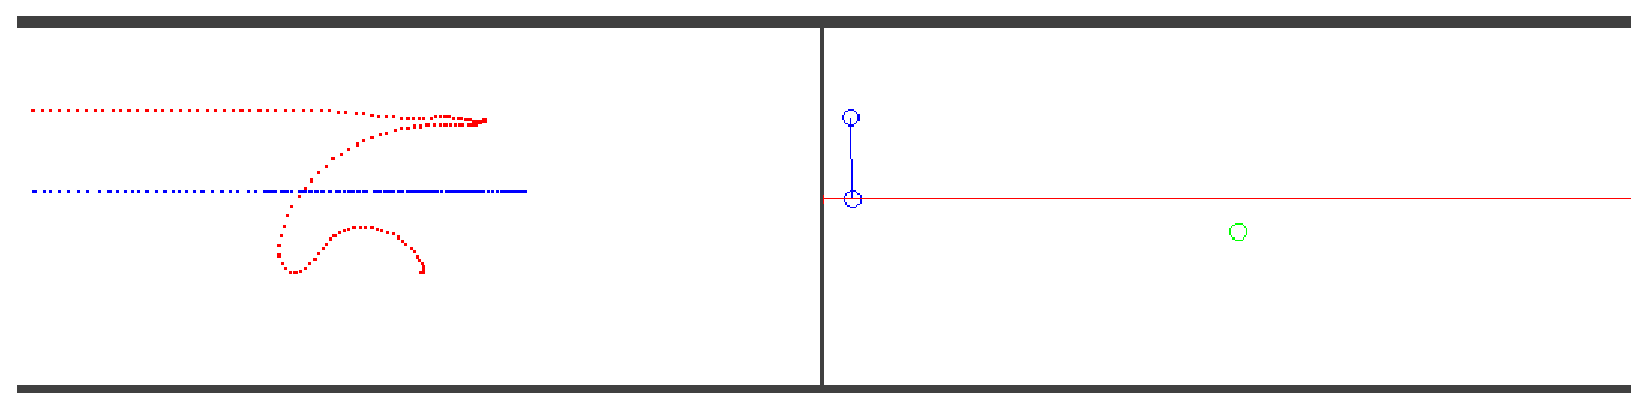
\epsfig{file=neuralfield-panel-2.eps, width=14cm}
  \caption{System dynamics with an evolved Neural Field Controller, at
    time $t=4$. Left: trace of the pendulum (cart in blue and pole tip
    in red). Right: snapshot of the animation at time $t$.}
  \label{fig:theta-pi}
\end{figure*}

\section{Conclusions}
The neural field controller architecture is a bit complex (in its
implementation) and its simulation slightly costly, but has some
notable advantages. The first one is its ability to self-compensate
or, equivalently, the stability of its natural dynamics, which is
attained after the setup of few parameters. The second one is its
suitability to the problem at hand, being able to solve it with a good
performance for low and mid perturbations without evolution.

The evolved controller performed better than the other two, is more
general because eliminates the need for manual conscious
parameterization and allows the designer to specify more precisely the
performance measure desired.

\bibliographystyle{abbrv} \bibliography{bibanot}

\end{document}
